\documentclass[11pt]{article}

\usepackage{amsmath, amssymb}
\usepackage{booktabs}
\usepackage{geometry}
\usepackage{tikz}
\usepackage{graphicx}

\geometry{margin=1in}

\title{Physics-Based Cutting Force Model for CNC Machining}
\author{Mechanical Engineering Plan Document}
\date{\today}

\begin{document}

\maketitle

\section{Objective}
Develop a physics-based model to predict cutting forces in CNC machining based on:
\begin{itemize}
    \item Material properties
    \item Tool geometry
    \item Cutting parameters (speed, feed, depth)
\end{itemize}

\section{Theoretical Framework}

\subsection{Cutting Force Model}
\begin{equation}
F = K_c \cdot A_c
\end{equation}

\subsection{Chip Thickness}
\begin{equation}
h(\phi) = f_z \sin(\phi)
\end{equation}

\subsection{Milling Force Components}
\begin{align}
F_t &= K_t \cdot b \cdot h \\
F_r &= K_r \cdot b \cdot h
\end{align}

\subsection{Material Dependence}
\begin{equation}
K_c = K_{c1.1} \cdot h^{-m}
\end{equation}

\subsection{Corrected Speed Relations}
\textbf{Imperial:}
\begin{equation}
RPM = \frac{SFM \cdot 3.82}{D}
\end{equation}

\textbf{SI:}
\begin{equation}
N = \frac{1000 \cdot V}{\pi D}
\end{equation}

\subsection{Feed Rate}
\begin{equation}
F = N \cdot Z \cdot f_z
\end{equation}

\section{Material Parameters (From Shop Data)}

\begin{table}[h!]
\centering
\begin{tabular}{lcc}
\toprule
\textbf{Material} & \textbf{SFM Range} & \textbf{Typical $K_c$ (MPa)} \\
\midrule
Aluminum (6061) & 800--1200 & 600 \\
Aluminum (cast) & 600--900 & 700 \\
Mild Steel (1018) & 300--500 & 1800 \\
Alloy Steel (4140) & 200--400 & 2200 \\
Stainless Steel (304) & 150--300 & 2400 \\
Tool Steel (D2) & 100--250 & 3000 \\
Cast Iron & 400--700 & 1600 \\
Brass & 500--1000 & 500 \\
Titanium (Ti-6Al-4V) & 80--200 & 3000 \\
Nickel Alloys (Inconel) & 50--150 & 3500 \\
\bottomrule
\end{tabular}
\caption{Cutting parameters derived from shop-floor tables [1]}
%(https://uofwaterloo-my.sharepoint.com/personal/sbedi_uwaterloo_ca/Documents/Microsoft%20Copilot%20Chat%20Files/feeds_speeds.pdf)}
\end{table}

\section{Practical Interpretation}

\begin{itemize}
    \item Feed controls chip thickness and force
    \item Speed controls temperature
    \item Depth controls total load
\end{itemize}

Key observation:
\begin{quote}
If chips are dust → feed too low \\
If chatter occurs → reduce feed first
\end{quote}
\textit{(Shop-floor rule)} 
%[1](https://uofwaterloo-my.sharepoint.com/personal/sbedi_uwaterloo_ca/Documents/Microsoft%20Copilot%20Chat%20Files/feeds_speeds.pdf)

\section{Simplified Force Model}
\begin{equation}
F \approx K_c \cdot f_z \cdot a_p \cdot a_e
\end{equation}

\section{Implementation Plan}

\subsection{Phases}
\begin{enumerate}
    \item Analytical model development
    \item Data collection (spindle load, cuts)
    \item Parameter identification
    \item Real-time CNC integration
    \item Adaptive optimization
\end{enumerate}

\section{System Flow Diagram}

\begin{center}
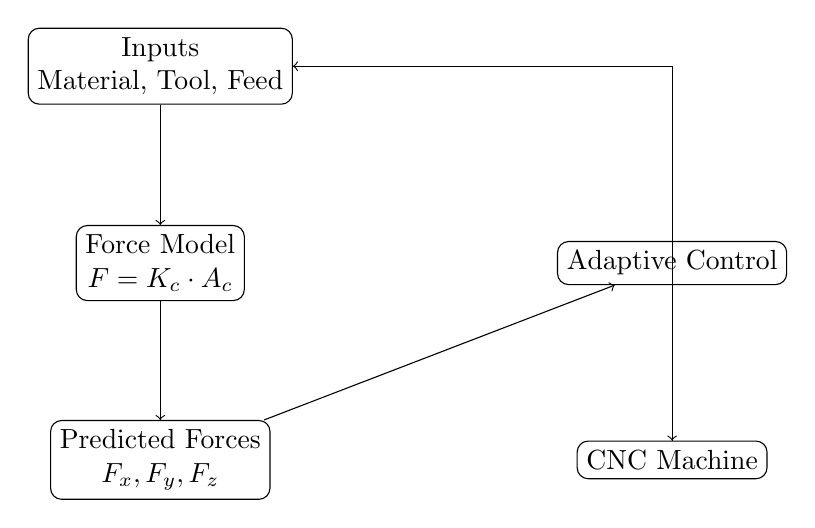
\begin{tikzpicture}[
    node distance=2.5cm,
    every node/.style={draw, rectangle, rounded corners, align=center}
]

\node (input) {Inputs \\ Material, Tool, Feed};
\node (model) [below of=input] {Force Model \\ $F = K_c \cdot A_c$};
\node (output) [below of=model] {Predicted Forces \\ $F_x, F_y, F_z$};
\node (control) [right of=model, xshift=4cm] {Adaptive Control};
\node (machine) [below of=control] {CNC Machine};

\draw[->] (input) -- (model);
\draw[->] (model) -- (output);
\draw[->] (output) -- (control);
\draw[->] (control) -- (machine);
\draw[->] (machine) |- (input);

\end{tikzpicture}
\end{center}

\section{Validation Plan}
\begin{itemize}
    \item Compare predicted vs measured forces
    \item Evaluate tool wear and chatter
    \item Validate across materials and operations
\end{itemize}

\section{Conclusion}
Cutting force is primarily governed by chip formation physics. 
A successful model integrates:
\begin{itemize}
    \item Mechanistic equations
    \item Empirical shop-floor adjustments
\end{itemize}

\end{document}